\documentclass[10pt]{article}
\usepackage{mathtools}
\usepackage{amsmath}
\usepackage{tabularx}
\usepackage{graphicx}
\usepackage{flexisym}
\usepackage{listings}
\usepackage[most]{tcolorbox}
\usepackage{xcolor}
\usepackage{hyperref}
\usepackage{amsthm}
\usepackage{subcaption}
\usepackage{hyperref}
\usepackage[a4paper,top=3cm,bottom=2cm,left=3cm,right=3cm,marginparwidth=1.75cm]{geometry}   
\newtcblisting[auto counter]{pseudolisting}[2][]{sharp corners,
    fonttitle=\bfseries, colframe=gray, listing only,
    listing options={basicstyle=\ttfamily,language=c++},
    title=Listing \thetcbcounter: #2, #1}

\newtheorem*{theorem}{Theorem}
\begin{document}
\setlength\parindent{1pt}
\title{Studies of phase transitions in magnetic systems}
\author{Andrei Kukharenka \\  
FYS 4150 
}

\maketitle
\begin{abstract}
In this project we study phase transitions in a magnetic system by using Ising model in two dimensions.
We use periodic boundary conditions and the Metropolis algorithm simulating phase transition by Monte Carlo methods.
Open MPI library used for code parallelization. Phase transition from ferromagnetic phase to diamagnetic can be clearly seen, however
finite size effects take place.
All the result are in a good agreement with the solutions obtained for the closed form. The critical temperature turned to be close to the exact result obtained by Lars Onsager. ​


\end{abstract}
\clearpage 


\section{Introduction}
Ising model is one of the most widely studied models in physics. It is extremely useful and precise when describing different kinds of magnetism: ferro, anti-ferro and ferrimagnetism. Ising model can show how competition between entropy and energy leads to phase transition. \\
In this work we use this widely popular model to simulate phase transitions. Monte Carlo methods is naturally to use due to the fact that our problem has a probabilistic interpretation.
We find the analytical expression for the partition function and various expectations values for simple 2$\times$2 case.
Then we present results obtained numerically by our program and compare results with ones obtained analytically for 2$\times$2 lattice.

To study phase transitions we parallelize code using MPI.

The report has the following structure:\\*
In the part \ref{Part1}  we discuss the problem and describe Ising model, then we briefly discuss random walks and Metropolis algorithm. Those who are already familiar with those methods and Ising model can safely skip this part and go directly to the results and discussion part \ref{results}. In conclusion \ref{conc} a brief overview of obtained results and discuss possibilities for further research are given. 

 

\newpage
\section{Problem formulation and mathematical method}\label{Part1}



\subsection{Ising model}
It is known that ferromagnetic materials have spontaneous magnetic moment that is not equal to zero at certain temperatures even with no external magnetic field applied. For readers not familiar with magnetic materials text of Kittel \cite{Kittel} chapter 12 is recommended.
In other words spins of electrons have some kind of ordering. We assume that interaction between spins exists inside magnetic material and 
this interaction can be described by some kind of quasi-magnetic field often called exchange field. Thermal agitation and exchange field are competitors and we can say that increasing temperature we can reach such a point where thermal energy will dominate and magnetic ordering will be destroyed.
In mean-field approximation it is assumed that $B_E$, exchange field is proportional to magnetization $M$:

\[
B_E \sim M
\]

So every spin can see only average magnetization of other spins. Bellow we introduce model and a method allowing us to calculate numerically critical temperature and 
magnetization of magnetic. \\
Let us modulate magnetic as two-dimentional square lattice. In general case it's possible to study other types of lattices and three-dimensional case, we employ 2D square lattice
just for simplicity here. We assume that the spin in every lattice point can have just two possible values, either pointing up (+1) or pointing down(-1). This simple approximation is
called Ising model, named after Ernst Ising who introduced this idea in early 1920s.

If one applies Ising model to a magnetic system employing mean field approximation energy can be written as:

\begin{equation}\label{isingenergy}
E=-J\sum_{\langle kl\rangle }^{N}s_{k}s_{l} - B\sum_{k}^{N}s_k
\end{equation}

where $N$ is number of spins, $J$ is a coupling constant that express interaction
strength between spins, $s_{k}=\pm 1$, $\langle kl\rangle $
means that sum is taken over neighboring spins only. $B$ is external magnetic field.
In this project we consider the only case without external magnetic field, so second term in equation (\ref{isingenergy}) is equal to zero.\\


From statistical physics we use canonical ensemble concept as our system exchange only heat. To calculate expectation values of energy and magnetization we need a probability distribution for discrete quantities:
\begin{equation}\label{expectations}
\begin{aligned}
\langle M \rangle =\frac {1}{N}\sum_{i=1}^{N} P(M_i)M_i \\
\langle E \rangle = \frac {1}{N}\sum_{i=1}^{N} P(E_i)E_i
\end{aligned}
\end{equation}
where $\langle M \rangle$ is mean magnetization, $\langle E \rangle$ -- mean energy,
$P(M_i),\ P(E_i)$ -- probability distribution for magnetization and energy, $N$ is number of microstates.
Probability distribution is given by Bolzmann distribution in our case:

\begin{equation}\label{Boltsmann}
P_i(\beta)=\frac {e^{-\beta E_i}}{Z},
\end{equation}

where $\beta = 1/k_BT$, $k_B$ -- Bolzmann constant, $T$ -- temperature, $Z$ is a partition function (or
normalization factor) for canonical ensemble defined as:

\begin{equation}\label{partfunc}
Z=\sum_{i}^{N}e^{-\beta E_{i}}
\end{equation}

Implying equations (\ref{Boltsmann}) and (\ref{partfunc}) it's easy to show that (\ref{expectations}) can be rewritten as:

\begin{equation}
\begin{aligned}
\langle E\rangle &=&\frac{1}{Z}\sum_{i}^{N}E_{i}e^{-\beta E_{i}} \\
\langle M\rangle &=&\frac{1}{Z}\sum_{i}^{N}M_{i}e^{-\beta E_{i}}
\end{aligned}
\end{equation}

where $N$ is number of microstates, $E_{i}$ energy of microstate $i$, $M_{i}$ -- magnetization of microstate $i$. 

Magnetic susceptibility and heat capacity can be calculated then as follows: 
\begin{equation}\label{cv_xi}
\begin{aligned}
C_{v}=\frac{\sigma^2 _{E}}{k_{B}T^{2}}=\frac{\langle E^{2}\rangle -\langle E\rangle ^{2}}{k_{B}T^2} \\
\chi =\frac{\sigma^2 _{M}}{k_{B}T}=\frac{\langle M^{2}\rangle -\langle M\rangle ^{2}}{k_{B}T}
\end{aligned}
\end{equation}

If we know partition function we can calculate all quantities describing system. If we have a system of 2$\times$2 spins where each spin can have just two values($\pm$ 1), then it is needed to calculate just $2^{2^{2}} = 2^4$ microstates. For a system 4$\times$4 it's just a $2^{16}$ configurations and for 10$\times$10 -- $2^{10000}$ which is quite complicated to compute or solve analytically. So we need to apply
However 2$\times$2 can be solved and used as a test of our program.



\subsection{Random walks and Metropolis algorithm}
Consider a random walker in one dimension. Walker can jump to the left or to the right as well as stay in current state that is not making a move. Let us try to imagine this process applied to a system represented by Ising model and evolving in time. We consider one-dimensional case for simplicity.
Let assume we start with microstate with a specific spin arrangement. By flipping one spin we obtain a new microstate. So in space of microstates we get two different points. Naturally that random walker makes moves in a space of microstates in our case.
Random walker can either accept or neglect the move or with other words system will keep
current state or will move to a new one. And probability of being in a certain state must be normalized:
\[
\sum_{i} {w_i(t)} = 1
\]
Markov chain is a process where next position is independent of the previous one what ca be mathematically expressed as:
\[
w_i(t+t_s)=\sum_{j} {W(j\rightarrow i)w_j(t)}
\]
where $t_s$ is time step, $w_i$ - PDF in a time $t+t_s$ in state $i$, $W(j\rightarrow i)$ is transition probability from state $j$ to state $i$. To understand what transition probability is one can consider example in the beginning of this section where random walker could jump in 1D space either to the right or to the left. In this case
$W(j\rightarrow i)=W_{ji}=1/2$, if points in space are near each other ($|i-j|=1$). For other cases transition probability is zero as random walker can't jump over points during one move.
$W_{ji}$ represent probability of moving from one microstate to another mictostate which is in general case is impossible to calculate especially for complex systems.


For Ising model in two dimensions considered above we can write:
\[
w_i(t) = \frac{e^{-\beta E}}{Z},
\]

where $Z$ cannot be computed for considered Ising model of size more then 2$\times$2 lattice as was mentioned above.

Let we model $W(j\rightarrow i)$ as a product of probabilities:

\[
W_i(t) = T(j\rightarrow i)A(j\rightarrow i),
\]
where $T(j\rightarrow i)$ represents probability of making a move from state $j$ to state$i$, $A(j\rightarrow i)$ -- probability of acceptance move from $j$ to $i$. So probability to move to a new state is $T(j\rightarrow i)A(j\rightarrow i)$ while probability to reject move is $(1 - A(j\rightarrow i))$. Making assumption that $T$ and $A$ are time independent and normalized:

\[
w_i(t+1) - w_i(t) = \sum_{j}{(w_j(t)T(j\rightarrow i)A(j\rightarrow i) - w_i(t)T(i\rightarrow j)A(i\rightarrow j))}
\]
In the limit where time goes to infinity $w_i(t+1)=w_i$ and $w_i(t)=w_i$, so last equation becomes:
\[
\sum_{j}{(w_j(t)T(j\rightarrow i)A(j\rightarrow i)} = \sum_{j} {w_i(t)T(i\rightarrow j)A(i\rightarrow j))}
\]
To avoid cyclic solutions and converge to the biggest eigenvalue(this is discussed in Chapter 11 of \cite{one}) we use detailed balance equation:
\[
W(j\rightarrow i)w_j=W(i\rightarrow j)w_i
\]
Which is leads to following equation:

\[
\frac{T(j\rightarrow i)A(j\rightarrow i)}{T(i\rightarrow j)A(i\rightarrow j)}=\frac{w_i}{w_j}
\]
As we mentioned above our system is described by Boltzmann distribution. So last equation can be rewritten as:
\[
\frac{w_i}{w_j} = exp(-\beta(E_i - E_j))
\]



Program implementing described method in not complicated one. Main algorithm can be expressed as following pseudocoding:
\begin{pseudolisting}{Metropolis pseudo-code for Ising model}
Start loop over temterature while (T <= T_finish){
 Calculate Energy and magnetization of the system
 Start Monte Carlo loop (one loop is N*N spin flips)
  flip one random spin
  calculate energy difference
  if (energy difference less or equal zero){
   accept move
   update MC_counter
  } else {
   call Random Number Generator(RNG)
   if (energy difference is less then RNG number){
    decline move (flip back spin)
    update MC counter
   } else {
    accept move
    update MC_counter
   }
  End Monte Carlo loop
  Update expectations
  Reset counters
  Add temperature step
End loop over temterature
\end{pseudolisting}

There is one note regarding optimization of program. Since we are going to run simulations for different lattices Monte Carlo loop calculations grows as squared lattice size. However we flip only one spin at the time, that means that we have only five different possible values of energy difference and we can precalculate them to speed up program. In program it is done by precalculate\_exp\_deltaE function:
\begin{pseudolisting}{precalculate\_exp\_deltaE}
for (int i=-8;i<=8;i+=4){
  exp_energy[i+8]=exp((double) -i/Temperature);
}

\end{pseudolisting}
Additionally we want to note that accuracy of expectation values depends on number of Monte Carlo cycles. Modern CPUs have several cores and it it naturally to think that one computer has several CPUs. In next section we discuss briefly how to run Monte Carlo experiments on one computer
parallel. 
\subsection{Parallelization}
In this section we will discuss how we can speedup our numerical experiment by parallelizing code with OpenMPI library \cite{Gabriel}. 
We divide our task into independent tasks each running Monte Carlo sampling. So for every temperature we run eight parallel experiments.
When all tasks are finished master process gets all expectation values sum them and writes to file.

\begin{pseudolisting}{Open MPI usage}
int numprocs, my_rank;
MPI_Init (&argc, &argv);
MPI_Comm_size (MPI_COMM_WORLD, &numprocs);
MPI_Comm_rank (MPI_COMM_WORLD, &my_rank);

Loop Over temperature {
    ...
  }

MPI_Reduce(&Xi, &m_Xi, 1, MPI_DOUBLE, 
          MPI_SUM, 0, MPI_COMM_WORLD);
MPI_Reduce(&Cv, &m_Cv, 1, MPI_DOUBLE, 
          MPI_SUM, 0, MPI_COMM_WORLD);
MPI_Reduce(&slave_E, &m_E, 1, MPI_DOUBLE, 
          MPI_SUM, 0, MPI_COMM_WORLD);
MPI_Reduce(&slave_M, &m_M, 1, MPI_DOUBLE, 
          MPI_SUM, 0, MPI_COMM_WORLD);

Master process writes to file

End of loop over temperature

\end{pseudolisting}




\section{Results and discussion}\label{results}

\subsection{2$\times$2 lattice}

For 2$\times$2 lattice it is needed to calculate just $2^4 = 16$ microstates. We used brute-force approach implying equation for energy (\ref{isingenergy}). Magnetization was calculated using following equation:
\[
M=\sum_{i=1}^{16} s_i
\]

Results are presented in Table \ref{tab:2x2}.

\begin{table}[h!]
  \caption{Values of energy and magnetization for two-dimensional Ising model of magnetic with square lattice. Lattice size is 2$\times$2. Periodic boundary conditions were used.}
  \label{tab:2x2}
  \begin{center}
    \begin{tabular}{c|c|c|c}
    \hline
		Number of spins up(+1) & Degeneracy & Energy, $J$ & Magnetization \\
        \hline
	$	0 $  & $ 1 $ & $ -8 $ & $ -4 $  \\
	$	1 $  & $ 4 $ & $  0 $ & $ -2 $  \\
	$	2 $  & $ 2 $ & $  8 $ & $ 0  $  \\
	$	2 $  & $ 4 $ & $  0 $ & $ 0  $  \\
	$	3 $  & $ 4 $ & $  0 $ & $ 2  $  \\
  $	4 $  & $ 1 $ & $  8 $ & $ 4  $  \\

	\end{tabular}
  \end{center}
\end{table}

 we can calculate the mean value of energy and
magnetization as well as heat capacity and magnetic susceptibility.
Closed form solution for partition function is:

\begin{equation}\label{pfun}
z=\sum_{i}^{M}e^{-\beta E_{i}}=\sum_{E}\Omega (E)e^{-\beta E}
\end{equation}

where $\sum_{E}$ is sum for all allowed energies, $\Omega (E)$ is degeneracy
for each energy. 

Using calculated energy for every microstate from Table \ref{tab:2x2} and (\ref{pfun}) it is easy to get a closed form solution for
partition function:

\begin{equation}
Z=2e^{-8\beta J}+2e^{8\beta J}+12=4\cosh (8\beta J)+12
\end{equation}

Expectation value for the energy in this case is following:

\[
\langle E\rangle =\frac{1}{Z}\sum_{i}^{N}E_{i}e^{-\beta E_{i}}=-\frac{%
\partial \ln Z}{\partial \beta }=-\frac{\partial \ln (4\cosh (8\beta J)+12)}{%
\partial \beta }
\]
resulting in:
\begin{equation}\label{2x2_energy}
\langle E\rangle=-8J\frac{\sinh 8J\beta }{\cosh 8J\beta +3}
\end{equation}

Expectation value for magnetization is:

\[
\langle \left\vert M\right\vert \rangle =\frac{1}{Z}\sum_{i}^{N}\left\vert
M_{i}\right\vert e^{-\beta E_{i}}=\frac{4e^{8\beta J}+8+8+4e^{8\beta J}}{z}=%
\]

\begin{equation}\label{2x2magnet}
\langle \left\vert M\right\vert \rangle=\frac{2(e^{8\beta J}+2)}{\cosh (8\beta J)+3}
\end{equation}
Taking into account (\ref{2x2magnet}) and (\ref{2x2_energy}), it is easy to obtain heat capacity and
magnetic susceptibility from (\ref{cv_xi}):

\[
C_{v}=\frac{\partial ^{2}\ln Z}{\partial\beta ^{2}}=8J\frac{\partial \ln (\frac{\sinh 8J\beta }{\cosh 8J\beta +3})}{\partial \beta },
\]
which can be simplified to:
\begin{equation}\label{2x2Cv}
C_{v}=128J^{2}\frac{1+3\cosh 8J\beta }{6\sinh 8J\beta +\sinh 16J\beta }
\end{equation}

Similarly for magnetic susceptibility:

\[
\chi=\frac{\sigma^2 _{M}}{k_{B}T}=\frac{\langle M^{2}\rangle -\langle M\rangle ^{2}}{k_{B}T}
\]

results into:
\begin{equation}\label{2x2chi}
\chi=\frac{8\beta (e^{8J\beta }+1)}{\cosh 8J\beta +3}-\left( \frac{2(e^{8\beta J}+2)}{\cosh (8\beta J)+3}\right) ^{2}
\end{equation}

Now using (\ref{2x2magnet}), (\ref{2x2_energy}), (\ref{2x2Cv}) and (\ref{2x2chi}) we can calculate different expectation values for 2$\times$2 lattice. Additionally we present results obtained numerically by program we developed in Table \ref{tab:2x2_compare}. Source code and benchmarks are available at 
\href{https://github.com/andrei-fys/fys4150/tree/master/Project_4/src/task_b_c}{Ising model} .


\begin{table}[h!]
  \caption{Values of energy, magnetization, heat capacity and magnetic susceptibility for two-dimensional Ising model of magnetic with square lattice for temperature $1K$ and $J=1$ . Lattice size is 2$\times$2. Periodic boundary conditions were used. Exact solution was obtained by equations (\ref{2x2magnet}), (\ref{2x2_energy}), (\ref{2x2Cv}) and (\ref{2x2chi}). }
  \label{tab:2x2_compare}
  \begin{center}
    \begin{tabular}{c|c|c|c|c|c}
    \hline
		MC samples & $\langle E\rangle$ & $\langle \left\vert M\right\vert \rangle$ & $C_{v}$ & $\chi$ & relative error, \% \\
        \hline
	$	Exact $ & $-7.9839$ & $ 3.9946 $ & $ 0.12859 $ & $ 0.016043 $ & - \\
	$	10^5 $  & $-7.982$ & $ 3.9939 $ & $ 0.144956 $ & $ 0.0186428 $ & 16.2 \\
	$	10^6 $  & $-7.98405$ & $ 3.99465 $ & $ 0.127362 $ & $ 0.0161074 $ & 0.401 \\
	$	10^7 $  & $-7.9839$ & $ 3.99464 $ & $ 0.12856 $ & $ 0.0160516 $ & 0.023 \\

	\end{tabular}
  \end{center}
\end{table}

Results from Table \ref{tab:2x2_compare} clearly show us that Monte Carlo simulation is quite precise. At $10^6$ simulations relative error for magnetic susceptibility is roughly $0.5 \%$. For $10^5$ simulations relative error is quite big, however this number of Monte Carlo samples can be used to qualitative analysis of systems behavior.\\
It's easy to see that energy converges much faster then magnetization for both temperatures. Possible reason for this is the fact that in our model range of magnetization change is almost twice as small as similar rabge for energy. 
Additionally one should remember that number of spin flips is proportional to size of lattice. For 2$\times$2 case it is easy to perform $10^7$ Monte Carlo experiments, however can be quite time consuming for lattice 100$\times$100, when each Monte Carlo cycle contains $10^4$ spin flips. 
In next section we study system of 20$\times$20 size and use $10^5$ Monte Carlo samples to examine behavior of the system at different temperatures. 

\subsection{20$\times$20 lattice}
In Figs. \ref{fig:energy_1k}-\ref{fig:magnetization_24k} we present results obtained for 20$\times$20 lattice with $10^5$ Monte Carlo samples for T=1 $k_BT/J$ and T=2.4 $k_BT/J$. Figs. \ref{fig:energy_1k}-\ref{fig:magnetization_1k} show that at low temperature system reaches steady state faster if initial state was state with spontaneous magnetization. So it makes sense to use ordered initial configuration for lower temperatures. 
It is easy to see that at lower temperature energy converges much faster as expected due to the fact that number of accepted energies is lower that follows from Boltzmann distribution. Additionally it can be seen from Fig. \ref{fig:prob1} which represents energy distribution in our Monte Carlo simulation. Gap on Fig. \ref{fig:prob1} can be explained by our model and fact we flip one spin at the time which results in just five possible values for energy difference. 

For higher temperatures where we may not have information about systems preferred state it can be useful to use steady state of a little bit lower temperature as initial configuration and wait some number of Monte Carlo cycles while new steady state established. In general case time of thermalization should be studied carefully but we skip it in this work and make it topic for further research. Here we just study time system needs to reach equilibrium roughly graphical. And it's easy to see from Fig. \ref{fig:energy_24k} that first 10 \% of Monte Carlo calculations can be skipped.
We studied behavior of expectation values for energy and magnetization at just two temperatures, however it's interesting to check thermolization time for temperatures near critical temperature of phase transition. Results presented in this section were obtained by program available at \href{https://github.com/andrei-fys/fys4150/tree/master/Project_4/src/task_d}{Ising model}. Following mentioned link information how to repsenent results can be found. We do not provide result files with dependencies of expectation on number of Monte Calro cycles due to file size. However instructions how to reproduce results are given.


\newpage
\begin{figure}
\centering
   \begin{subfigure}[b]{1\textwidth}
   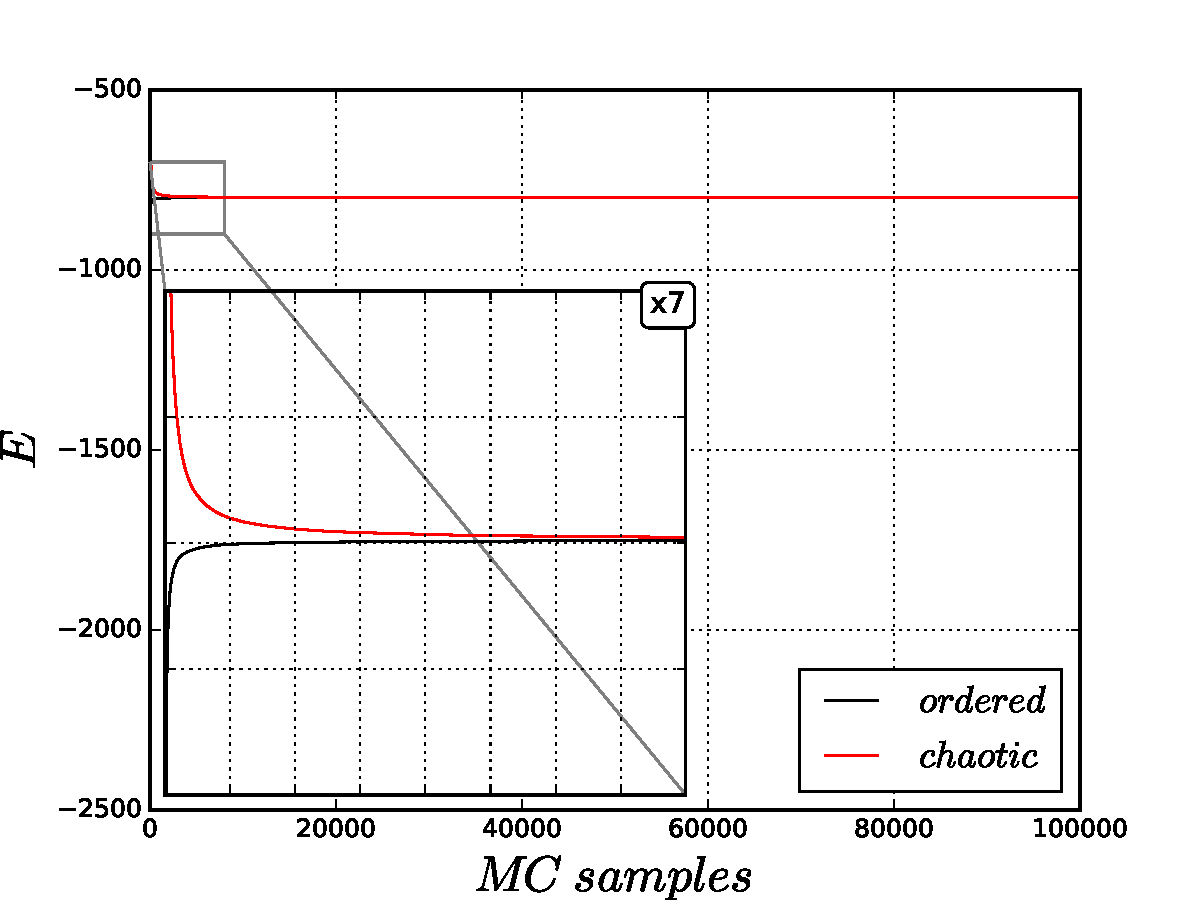
\includegraphics[width=0.9\linewidth]{20x20_10_5_1_energy}
   \caption{Energy, L = 20$\times$20, T = 1 $k_BT/J$.}
   \label{fig:energy_1k} 
\end{subfigure}

\begin{subfigure}[b]{1\textwidth}
   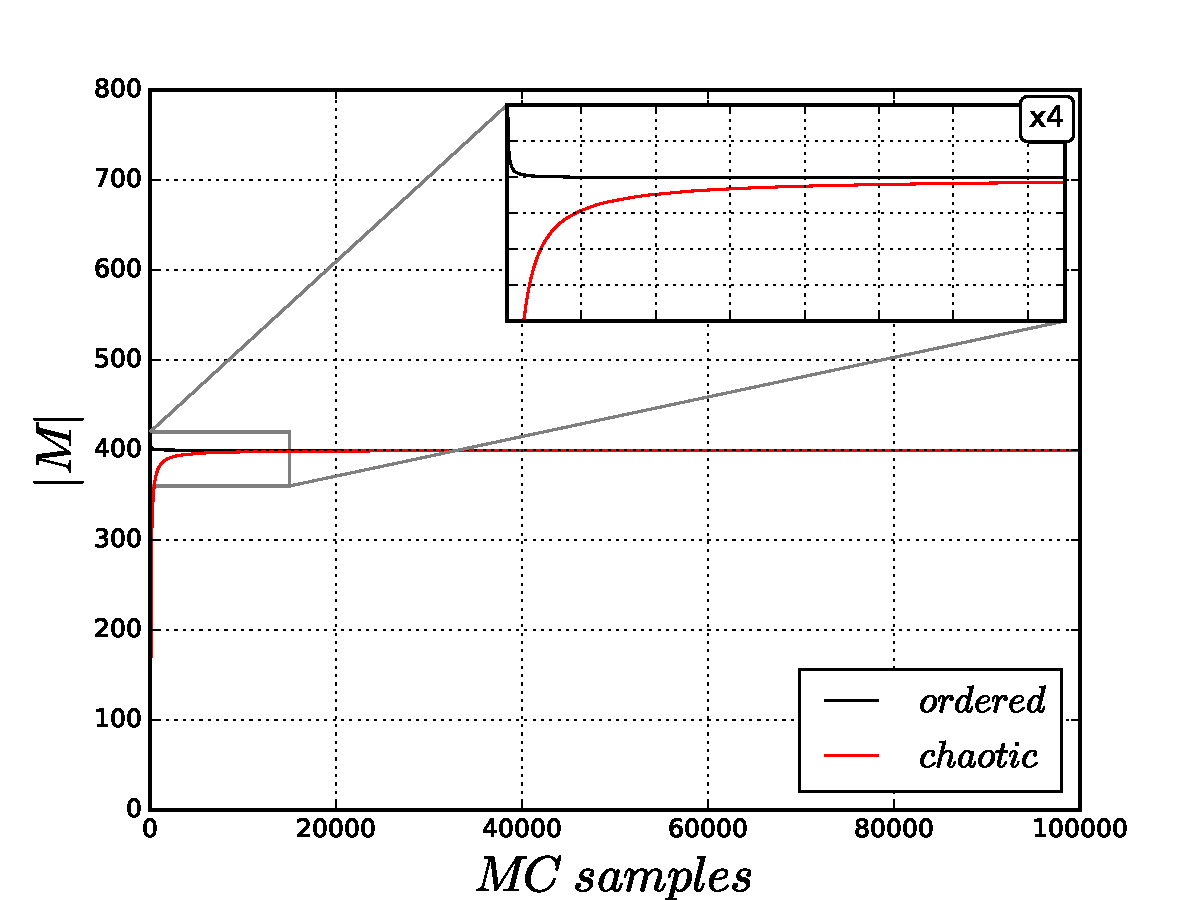
\includegraphics[width=0.9\linewidth]{20x20_10_5_1_magnet}
   \caption{Magnetization, L = 20$\times$20, T = 1 $k_BT/J$.}
   \label{fig:magnetization_1k}
\end{subfigure}

\caption[Two numerical solutions]{Expectations values of mean energy (a)  and absolute value of mean magnetization (b) as functions
of the number of Monte Carlo cycles for system of 20$\times$20 spins at T=1 $k_BT$. $10^5$ Monte Carlo samples were used in calculations.
Both an ordered and a random spin orientation as initial configuration were used in calculations.}
\end{figure}

\clearpage
% \begin{figure}
%Histograms instead.
%   \centering
%     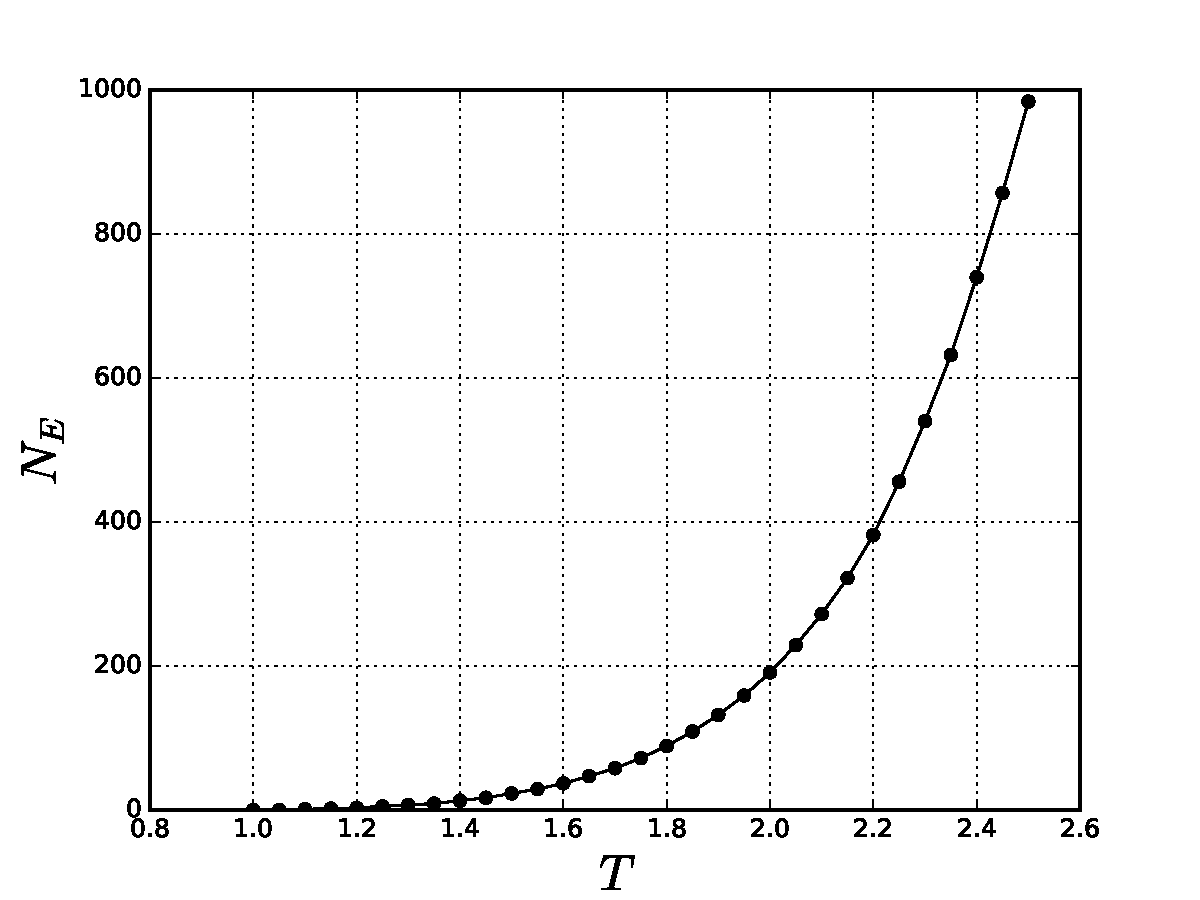
\includegraphics[width=1\linewidth]{accepted}
%     \caption{Numerical($V_i$) and exact($U_i$) solutions plotted for $100$ grid points. The numerical solution was obtained by Gauss elimination algorithm. To show the difference between numerical and exact solution at given grid size we represent magnified(12 times) part of a graph.}
%     \label{fig:gauss100}
% \end{figure}
%





\newpage
\begin{figure}
\centering
   \begin{subfigure}[b]{1\textwidth}
   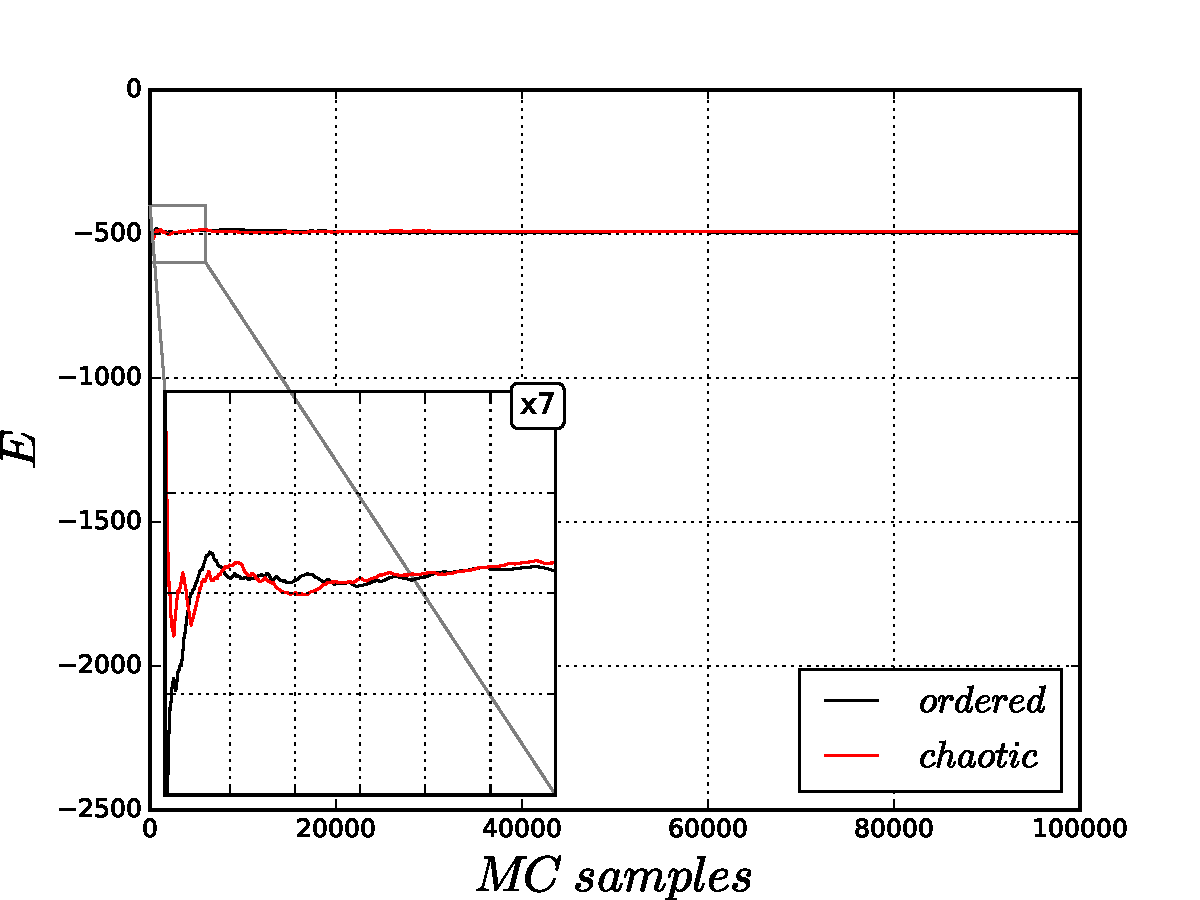
\includegraphics[width=0.9\linewidth]{20x20_10_5_24_energy}
   \caption{Energy, L = 20$\times$20, T = 2.4 $k_BT/J$.}
   \label{fig:energy_24k} 
\end{subfigure}

\begin{subfigure}[b]{1\textwidth}
   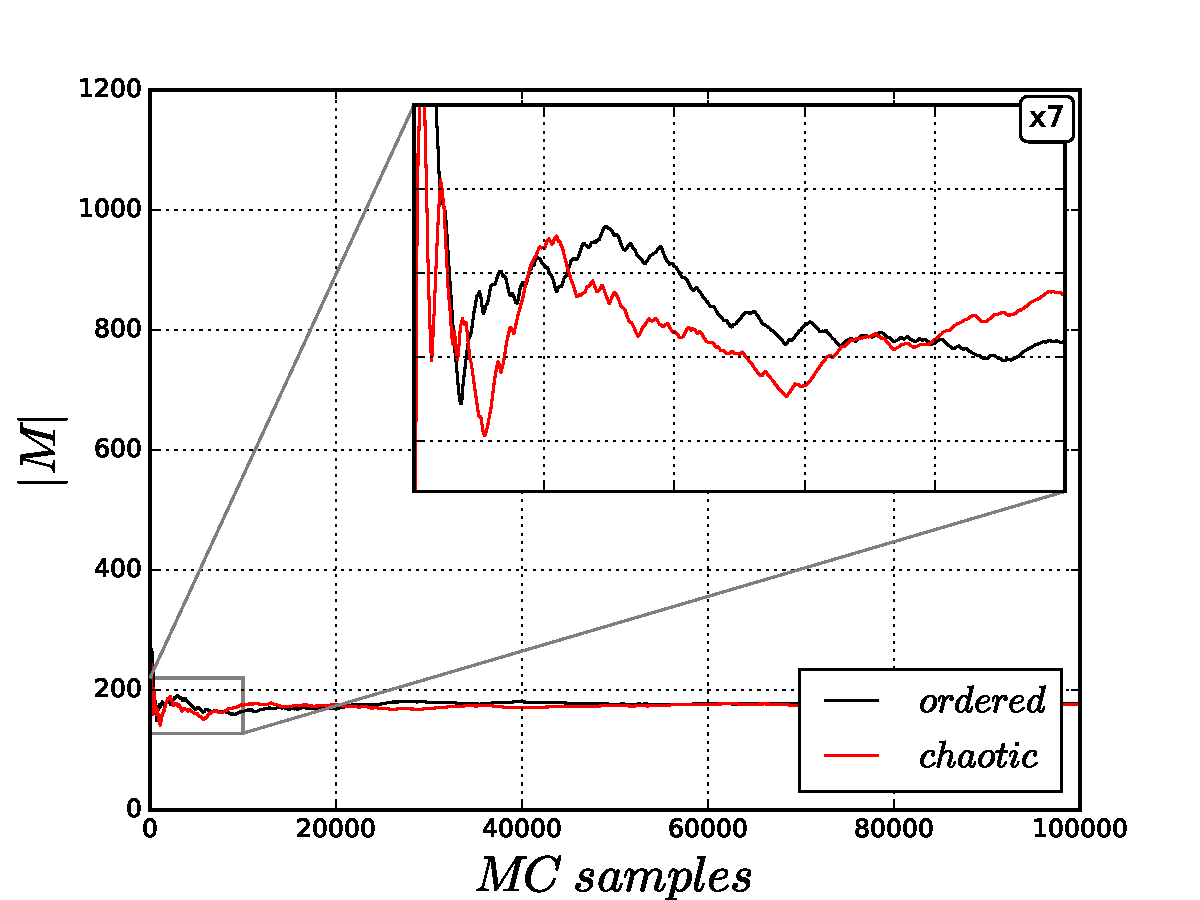
\includegraphics[width=0.9\linewidth]{20x20_10_5_24_magnet}
   \caption{Magnetization, L = 20$\times$20, T = 2.4 $k_BT/J$.}
   \label{fig:magnetization_24k}
\end{subfigure}

\caption{Expectations values of mean energy (a) and absolute value of mean magnetization (b) as functions
of the number of Monte Carlo cycles for system of 20$\times$20 spins at T=2.4 $k_BT/J$. $10^5$ Monte Carlo samples were used in calculations. 
Both an ordered and a random spin orientation as initial configuration were used in calculations.}
\end{figure}

\clearpage

\newpage
\begin{figure}
\centering
   \begin{subfigure}[b]{1\textwidth}
   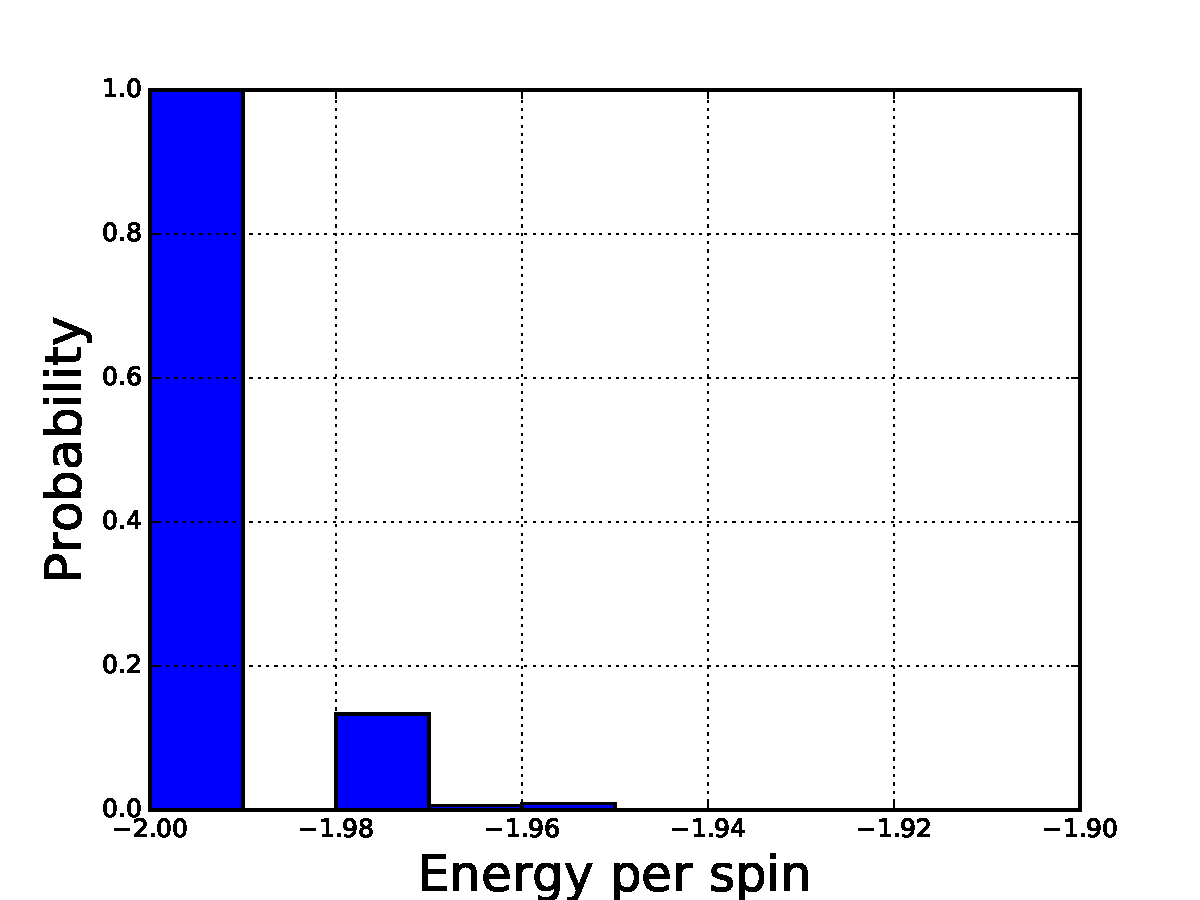
\includegraphics[width=0.9\linewidth]{Energy_pdf_20_T_1}
   \caption{Energy PDF at T = 1 $k_BT/J$.}
   \label{fig:prob1} 
\end{subfigure}

\begin{subfigure}[b]{1\textwidth}
   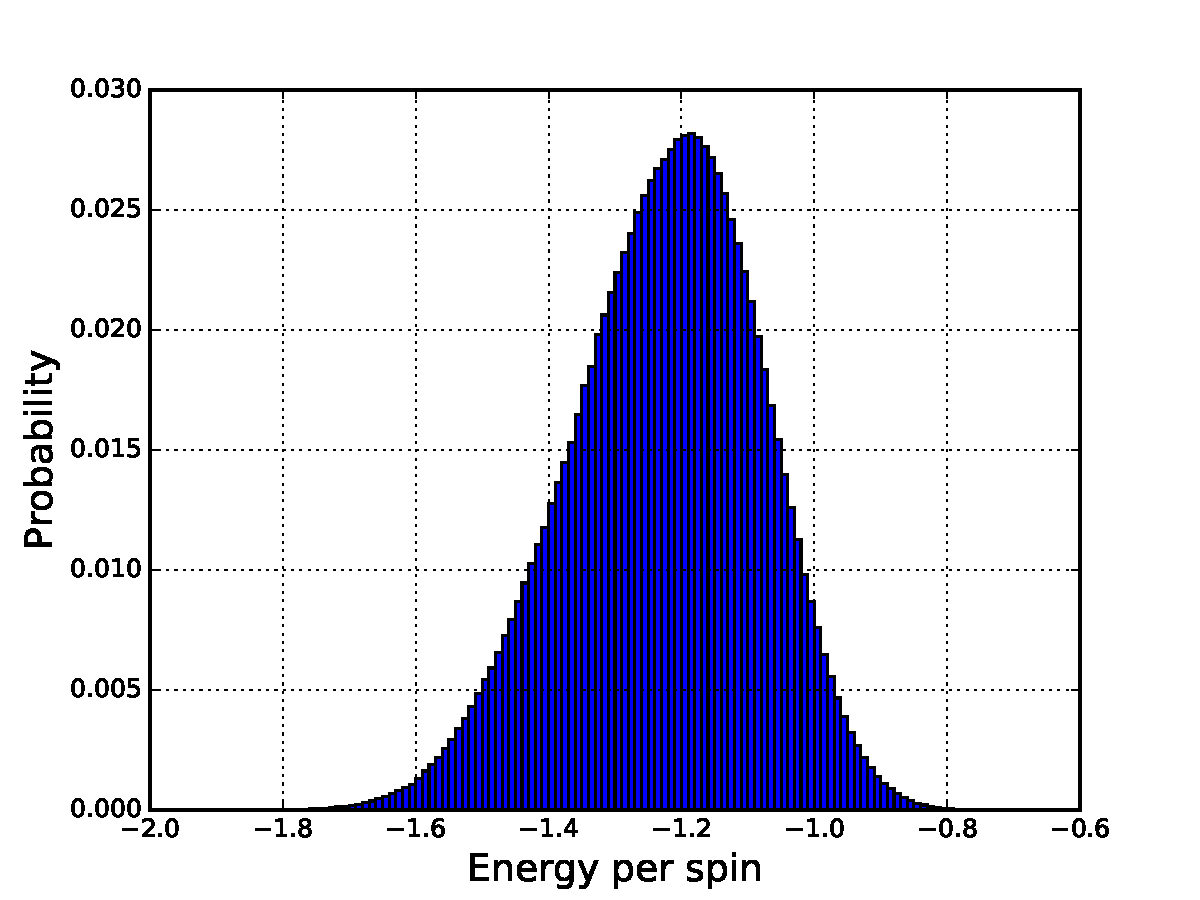
\includegraphics[width=0.9\linewidth]{Energy_pdf_20_24}
   \caption{Energy PDF at T = 2.4 $k_BT/J$.}
   \label{fig:prob24}
\end{subfigure}

\caption{Probability distribution of energy for system of 20$\times$20 spins at 1 (b) and 2.4 (a) temperatures.
Temperature is in units of $k_BT/J$. $10^5$ Monte Carlo samples were used in calculations.}
\end{figure}
\clearpage


\newpage

\subsection{Numerical studies of phase transitions}
In Figs. \ref{fig:phase_energy}-\ref{fig:phase_heat_cap} we present results obtained for 40$\times$40, 60$\times$60, 100$\times$100 and 140$\times$140 lattices in temperature range between 2.0 $k_BT/J$ and 2.41 $k_BT/J$ with $10^6$ Monte Carlo cycles and temperature step of 0.01. Fig. \ref{fig:phase_magnetiz} and fig:phase_magnetiz shows that phase transition takes place. Magnetization goes to zero, corresponding phase transition from ferromagnetic phase to diamagnetic. Magnetic susceptibility grows at the same temperature, similar effect is seen for heat capacity \ref{fig:phase_heat_cap}. We cannot observe that susceptibility goes to infinity due to finite lattice effects.
We use finite size scaling relations from \cite{one} to relate the behavior at finite lattices with the results for
an infinitely large lattice.
\[
T_c(L) - T_c(L = \infty ) = a L^{-1},
\]
where $T_c$ is critical temperature, $L$ is lattice size. Choosing $L=140$ and $L=100$ we got result that is $0.6$ \% differs from exact result for the critical temperature after \cite{Onsager}.
Source code of program used is provided on \href{https://github.com/andrei-fys/fys4150/tree/master/Project_4/src/MPI}{Ising model MPI} link.
Additionally results for $10^5$ Monte Carlo samples provided on same link. Simulations with $10^6$ cycles run for a considerable time on one computer. It took roughly two days on Intel(R) Core(TM) i7-3615QM CPU @ 2.30GHz with eight treads, so supercomputing facilities should be considered for fast reproduction of presented results. 




\begin{figure}
\centering
   \begin{subfigure}[b]{1\textwidth}
   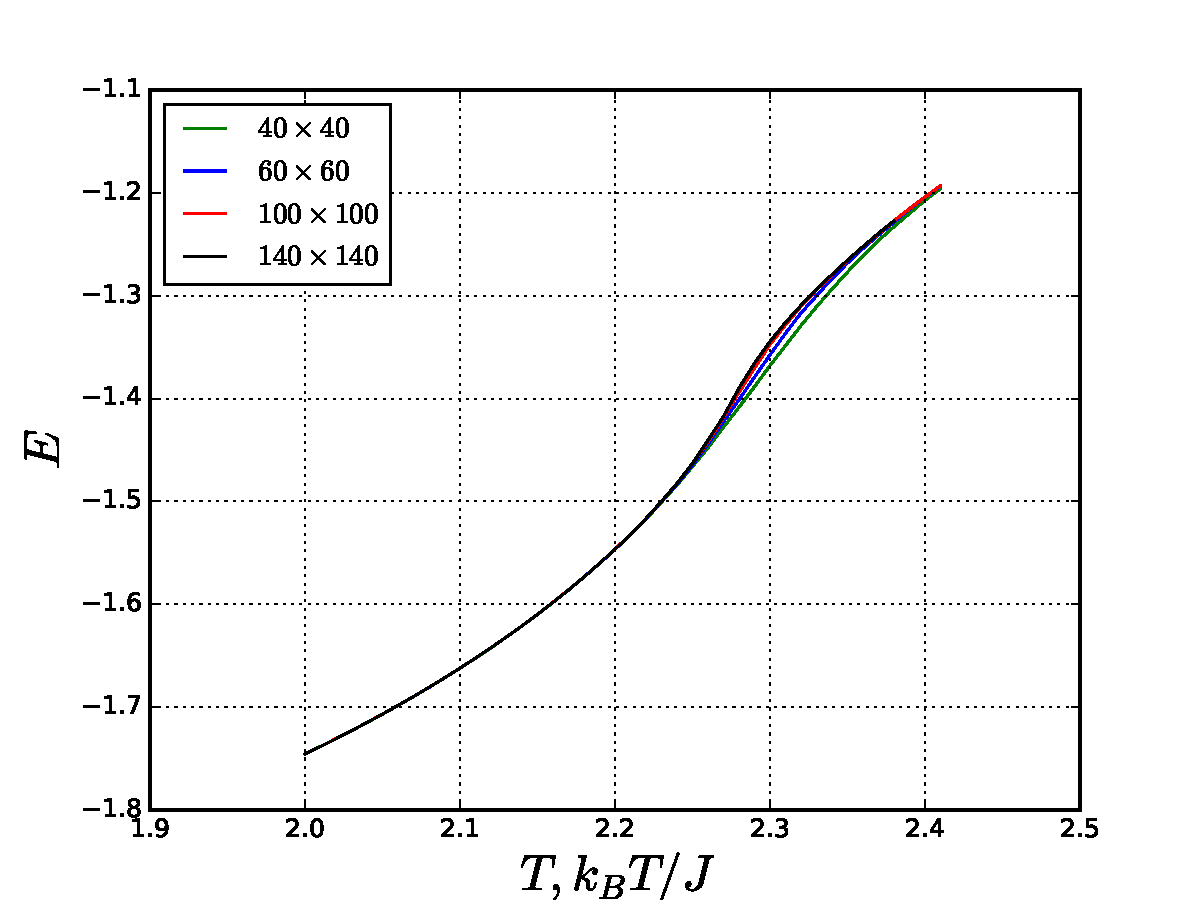
\includegraphics[width=0.9\linewidth]{phase_10_6_energy}
   \caption{Energy per spin.}
   \label{fig:phase_energy} 
\end{subfigure}

\begin{subfigure}[b]{1\textwidth}
   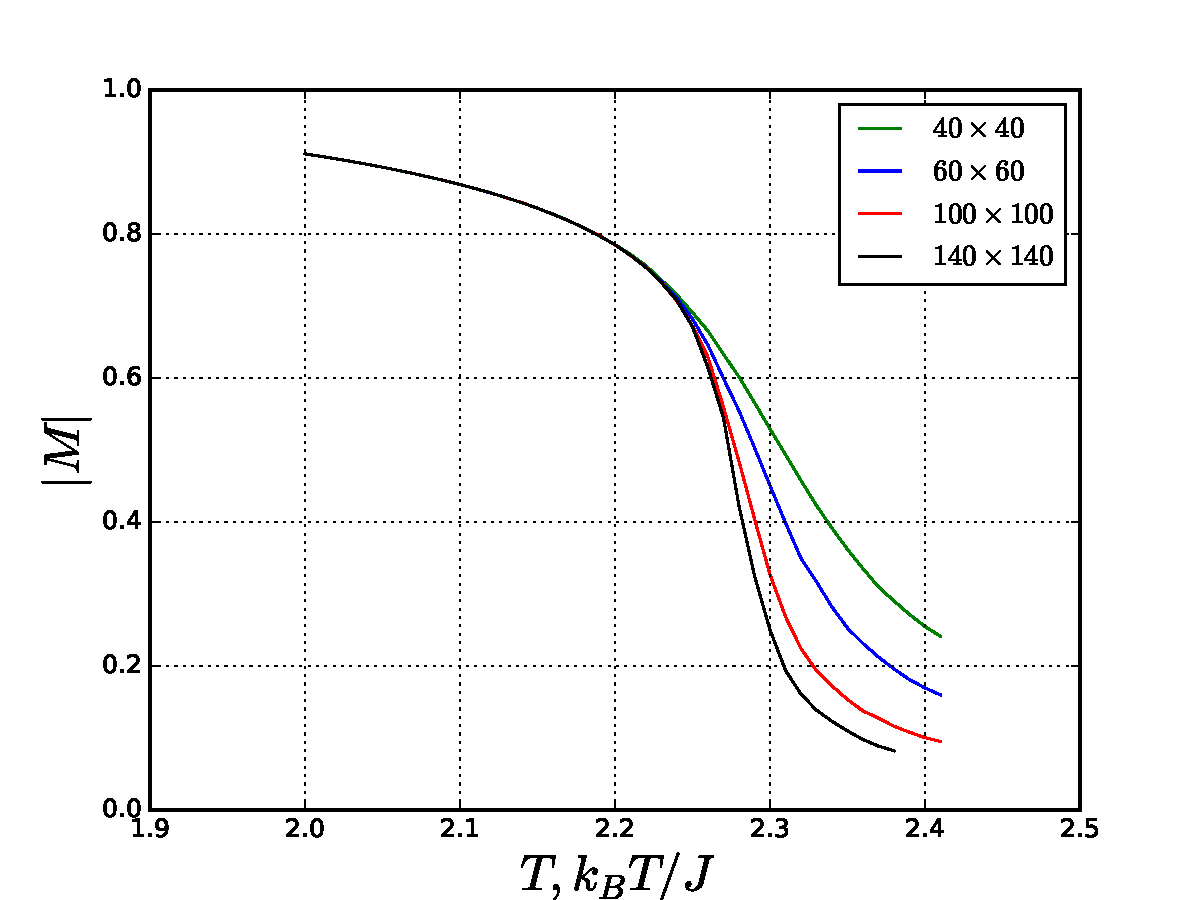
\includegraphics[width=0.9\linewidth]{phase_10_6_magnetization}
   \caption{Magnetization per spin.}
   \label{fig:phase_magnetiz}
\end{subfigure}
\caption{Energy (a) and Magnetization (b) for system of 40$\times$40, 60$\times$60, 100$\times$100 and 140$\times$140 spins
Temperature step is 0.01 $k_BT/J$. $10^6$ Monte Carlo samples were used in calculations.}
\end{figure}
\clearpage

\newpage
\begin{figure}
\centering
   \begin{subfigure}[b]{1\textwidth}
   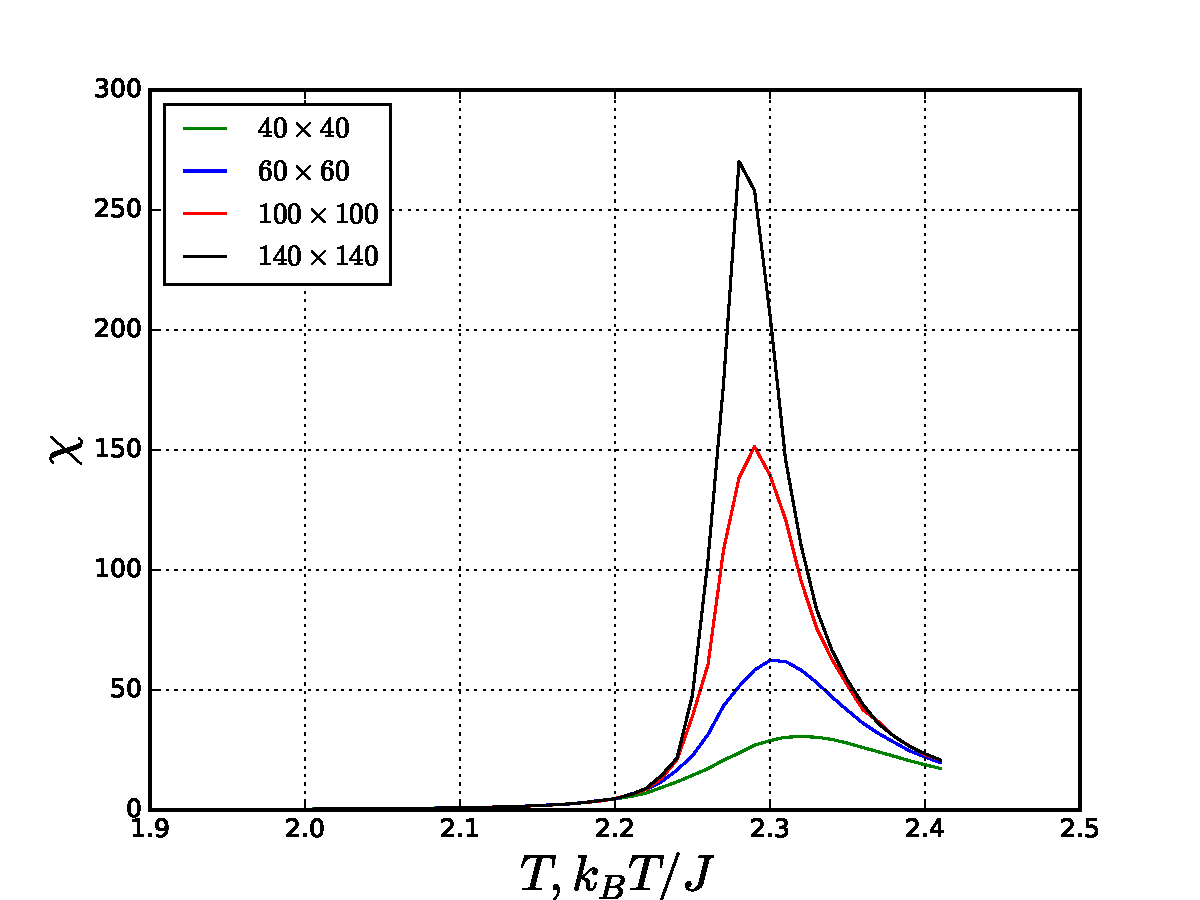
\includegraphics[width=0.9\linewidth]{phase_10_6_susceptability}
   \caption{Magnetic susceptibility per spin.}
   \label{fig:phase_suscept} 
\end{subfigure}

\begin{subfigure}[b]{1\textwidth}
   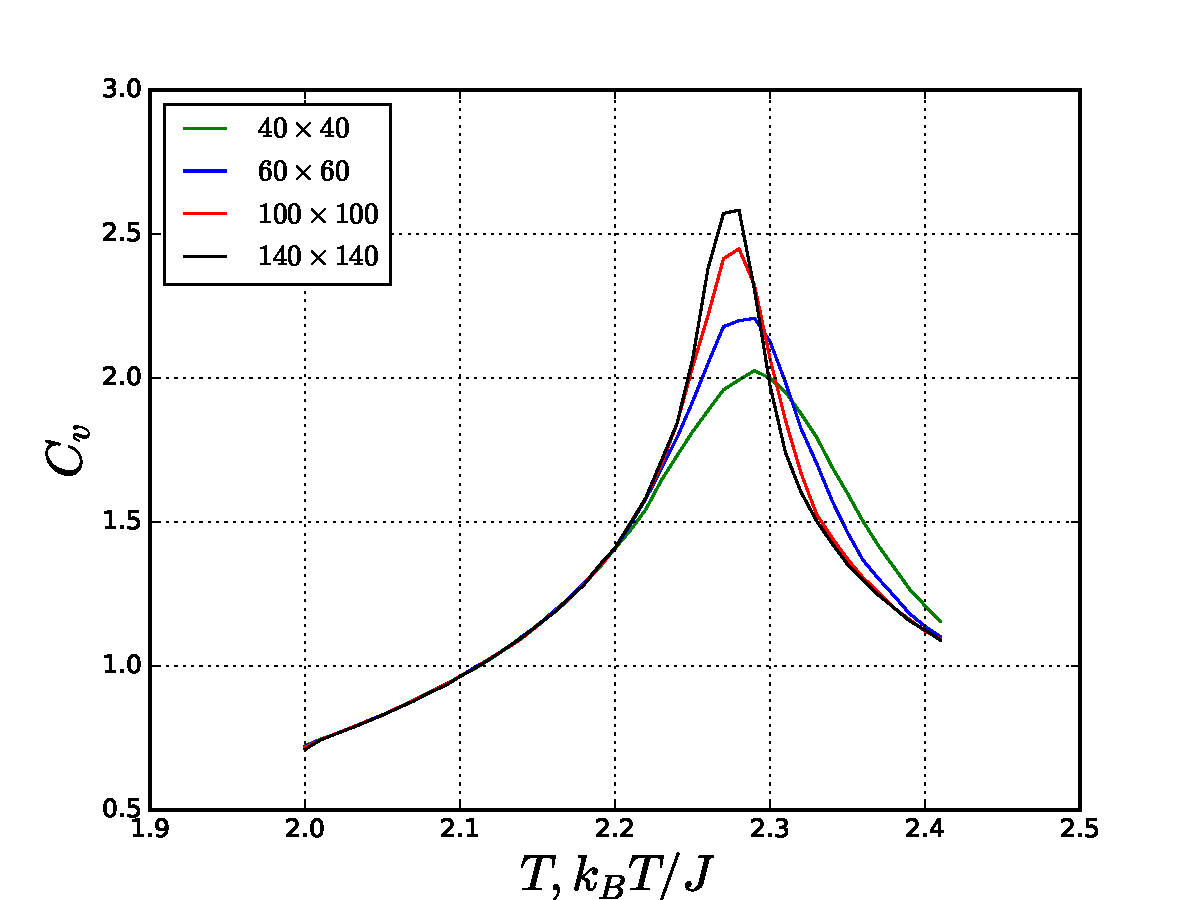
\includegraphics[width=0.9\linewidth]{phase_10_6_heat_capacity}
   \caption{Heat capacity per spin.}
   \label{fig:phase_heat_cap}
\end{subfigure}

\caption{Magnetic susceptibility (a) and heat capacity (b) for system of 40$\times$40, 60$\times$60, 100$\times$100 and 140$\times$140 spins
Temperature step is 0.01 $k_BT/J$. $10^6$ Monte Carlo samples were used in calculations.}
\end{figure}

\clearpage





\section{Conclusion and further research}\label{conc}
\newpage
\begin{thebibliography}{2}
\bibitem{one} 
Morten Hjorth-Jensen. 
\textit{Computational Physics
}. 
Lecture Notes Fall 2015, August 2015.

\bibitem{two} 
W. Press, B. Flannery, S. Teukolsky, W. Vetterling. 
\textit{Numerical Recipes in C++, The art of scientific Computing}. 
Cambridge University Press, 1999.

\bibitem {Kittel}
C. Kittel. 
\textit{Introduction to Solid State Physics}. 
Wiley, 2005.

\bibitem{Gabriel}
E. Gabriel,  Graham E. Fagg and others.
\textit{OpenMPI: Goals, Concept, and Design of a Next Generation MPI Implementation}
Proceedings, 11th European PVM/MPI Users' Group Meeting, 2004

\bibitem{Onsager}

\textit{Crystal Statistics. I. A Two-Dimensional Model with an Order-Disorder Transition}
Phys. Rev. 65, 117, 1944
\end{thebibliography}

\end{document}
